% ============================================================================
% III. PROBLEM, OBJECTIVE AND CONTROLLERS
% Equations, definitions, the controller table and the algorithms are written
% in full (permitted). Connecting prose is author-written (\todo).
% Implementation sources: controller/baselines/_objective.py (v1 shared
% terms), ours.py, b9_decomposed.py, b8_independent.py, b4_flare.py,
% b6_dragin.py; v2: _objective_v2.py, ours_v2.py, b9_v2.py, b9plus_v2.py,
% controller/sequential_v2.py; pseudocode source docs/research_v2/pseudocode.md.
% ============================================================================
\section{Problem Formulation and Controllers}\label{sec:problem}

% ---- P-III.1 ----------------------------------------------------------------
% PURPOSE: the decision a controller takes per turn.
% CLAIMS: a turn is a stream of ASR partials; at each partial the controller
%   may dispatch retrieval, wait, or (at end of turn) skip.
% One figure: fig_framework.pdf (paper_v2/tools/make_fig_framework.py),
% re-added on PI request 2026-10-18 (R1.f1, R2.10); block copied from
% sections/03_problem_draft.tex.
% Compact draft text: sections/03_problem_draft.tex.
\todo{P-III.1: the per-turn decision (Fig.~\ref{fig:system_flow}).}

\begin{figure*}[t]
\centering
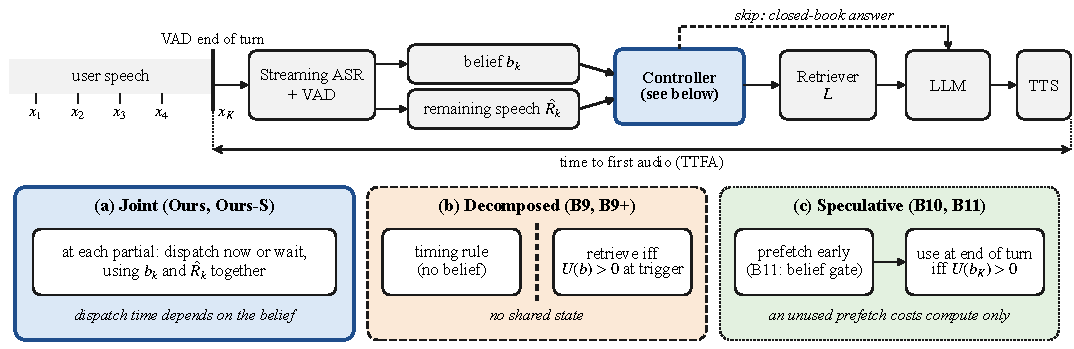
\includegraphics[width=\textwidth]{fig_framework.pdf}
\caption{Streaming pipeline and the decision structures compared. From each
ASR partial $x_k$ the system estimates the belief $b_k$ and the remaining
speech $\hat R_k$. (a) The joint controller decides at every partial whether
to dispatch now or wait. (b) Decomposed controllers fix the trigger without
the belief. (c) Speculative controllers prefetch early and decide at the end
of the turn whether to use the result.}
\label{fig:system_flow}
\end{figure*}


\subsection{Belief}\label{sec:belief}
% ---- P-III.2 ----------------------------------------------------------------
% PURPOSE: define the belief and say exactly what it is computed from.
% CLAIMS + EVIDENCE:
%   (a) v1 (Eq. belief-v1): s is the mean per-token entropy of a closed-book
%       draft generated from the FULL question x, averaged over 5 draws
%       (seeds 11,23,37,53,71, temperature 0.2, top-p 0.9, 80 tokens),
%       computed once per scenario before the sweep
%       [simulator/e3_scenario_signals.json "precompute"].
%       Hence the v1 belief does not depend on dispatch time (A3), even for
%       policies that dispatch before the question is complete (R1.4).
%   (b) The closed-book pass has a latency cost that v1 did not charge:
%       closed-book draft (80-token cap, Mistral-7B, isolated dev timing
%       run, 80 calls on 20 items per dataset): median TTFT 595 ms (d1_open)
%       / 596 ms (d2_support), median full generation 2,610 ms / 3,200 ms
%       [llm/experiment1_v2/results/<ds>/mistral7b_v03/latency_dev.jsonl;
%       docs/research_v2/paper_numbers_v2.json e1_latency_dev]. v2 charges
%       the belief's cost: its belief is the self-assessment probe, not the
%       draft, and every belief becomes available a median 548 ms (d1_open)
%       / 544 ms (d2_support) after its partial (one-token probe latency,
%       same run: self_assessment_latency_dev.jsonl; this is sa_lag_ms in
%       docs/research_v2/v2_predictions.json inputs).
%   (c) v2 (Eq. belief-v2): the belief is NOT draft entropy. It is the
%       calibrated self-assessment probe: SA_k = P("No") to the frozen
%       prompt sa-v1-frozen ("answerable from general knowledge alone,
%       without {org}'s own policies...? Yes/No"), read from Mistral-7B's
%       token probabilities and recomputed on each ASR partial x_k
%       [PRE2 H-E1v2; CONTRACTS Sec. 5--6]; calibrated as
%       b_k = sigmoid(a + b logit(SA_k) + c f_k + d logit(SA_k) f_k), f_k the
%       spoken word fraction, fitted on dev per dataset
%       [controller/baselines/e3v2_calibration_<ds>_mistral7b_v03_self_assessed_need_logit.json].
%   (d) Calibration: v1 is a logistic fit of P(need) on E1's 180 samples
%       (36 items x 5 seeds), IN-SAMPLE (R1.5); slope 11.288, intercept
%       -3.633; floor beta = 0.05 [configs/e3_price_grid.json calibration;
%       controller/baselines/e1_calibration_mean_entropy.json]. v2 fits
%       Eq. belief-v2 on the dev split only, per dataset, and evaluates on
%       test [PRE2 H-E1v2].
% NUMBERS: slope 11.288, intercept -3.633, floor 0.05, n = 180.
\todo{P-III.2: what the belief is computed from in v1 (draft entropy on the
full question, Eq.~(\ref{eq:belief})) and in v2 (the calibrated
self-assessment probe on each partial, Eq.~(\ref{eq:belief-v2})), the
in-sample v1 calibration versus the dev-only v2 calibration, and the
closed-book latency cost.}

\begin{equation}
s=\frac{1}{N}\sum_{i=1}^{N}H\!\left(p_\theta(\cdot\mid y_{<i},x)\right),\qquad
b=\max\!\big(\beta,\ \sigma(w\,s+c)\big)\qquad\text{(v1)},
\label{eq:belief}
\end{equation}
where $x$ is the full question, $y$ is the closed-book draft, $H$ is the
entropy in nats, $\sigma$ the logistic function and $\beta=0.05$ a floor.
In v2 the belief at step $k$ is
\begin{equation}
b_k=\sigma\!\big(a+b'\,\ell_k+c'\,f_k+d\,\ell_k f_k\big),\qquad
\ell_k=\operatorname{logit}(\mathrm{SA}_k)\qquad\text{(v2)},
\label{eq:belief-v2}
\end{equation}
where $\mathrm{SA}_k$ is the generator's probability of answering ``No''
to a fixed self-assessment prompt (can the question be answered from
general knowledge alone?) given the ASR partial $x_k$, $f_k$ is the spoken
word fraction, and $a,b',c',d$ are fitted on the dev split of each dataset.

\subsection{Objective}\label{sec:objective}
% ---- P-III.3 ----------------------------------------------------------------
% PURPOSE: define the corrected objective and say why the v1 form conflated
%   two quantities (R1.6): v1 used Q(retrieve) = b, i.e. it treated the
%   probability of need as the size of the gain and assumed retrieval never
%   hurts. Eq. (obj) separates P(need) = b from the gain g^+ on needed turns
%   and the harm g^- on non-needed turns.
% CLAIMS + EVIDENCE:
%   (a) On v1, retrieval raises accuracy from 0.112 to 0.832 on needed
%       scenarios (g^+ = 0.720 [0.504, 0.888]) and lowers it from 0.704 to
%       0.112 on non-needed ones (g^- = 0.592 [0.408, 0.768]); 25+25
%       scenarios x 5 seeds; scenario-bootstrap 95% CIs
%       [V1T retrieval_effect; cross-check PN e3_retrieval_effect].
%   (b) The zero-price retrieve boundary moves from b* = 0.05 (v1) to
%       b* = g^-/(g^+ + g^-) = 0.451 [V1T retrieval_effect.b_star_at_zero_cost].
%   (c) g^+, g^- are dataset-specific and are re-estimated on the v2 dev
%       split (primary ASR condition; final-transcript dispatch vs skip,
%       per-item mean over 5 seeds; docs/research_v2/v2_predictions.json
%       inputs.<ds>.g): d1_open g^+ = 0.441, g^- = -0.112 (877 needed /
%       689 not needed; a NEGATIVE harm, i.e. retrieval slightly helped
%       non-needed d1 items on dev, so b* < 0); d2_support g^+ = 0.445,
%       g^- = 0.034 (175 / 47; d2 dev uses judge-graded labels,
%       exploratory). text150 condition: d1 0.718 / 0.023, d2 0.463 / 0.166.
% NUMBERS: 0.112, 0.832, 0.704, 0.112, 0.720 [0.504, 0.888],
%   0.592 [0.408, 0.768], 0.451 -- all [V1T].
\todo{P-III.3: the corrected objective, why $Q=b$ was a conflation, and the
measured $g^{\pm}$.}

\begin{equation}
U_t(b)=b\,\gp(1-\rho_t)-(1-b)\,\gm-\lamL\,e_t-\lamC(1+w_t),\qquad U(\text{skip})=0,
\label{eq:obj}
\end{equation}
where $t$ is the dispatch timing, $\rho_t$ the fraction of $\gp$ lost to a
partial query, $e_t$ the expected exposed latency, $w_t$ the expected wasted
retrievals, and $\lamL$ (accuracy per second) and $\lamC$ (accuracy per
retrieval) are prices. The v1 objective is the special case $\gp=1$,
$\gm=\rho_t=0$, $e_t=L-o_t$ with a constant overlap $o_t$ per policy.
In v2 the exposure is turn-dependent,
\begin{equation}
e_k=\E\!\left[\pi+\max(0,\,L-W_k)\mid Z_k\right],
\label{eq:exposure}
\end{equation}
where $L$ is the retrieval latency, $W_k$ the speech remaining after step $k$
plus end-of-turn detection delay, $\pi$ the non-hideable part of retrieval's
cost (e.g.\ the longer prompt), and $Z_k$ the timing state observed at $k$.
Time to first audio is
\begin{equation}
\mathrm{TTFA}=t_{\text{first audio}}-t_{\text{user end}}.
\label{eq:ttfa}
\end{equation}

% ---- P-III.4 ----------------------------------------------------------------
% PURPOSE: say that waste_rate w_t is a placeholder in v1 (0, 0.02, 0.08)
%   that was never measured, and how v2 treats it (R1.10, R2).
% CLAIMS + EVIDENCE:
%   (a) v1 placeholder values [controller/baselines/_objective.py waste_rate;
%       paper/preregistration.md "Methodological Disclosures" item 2].
%   (b) In v1 all 751 logged retrievals had forecast_invalidated = false on
%       the text path, which cannot evidence the rate
%       [_objective.py waste_rate docstring].
%   (c) The exact price map depends on w through lambda_c (w* - w_se)/L
%       (Prop. 1); the approximate map lambda (L - o*)/L fails at 46 of 200
%       prices because of this term [V1T prop1_dense].
%   (d) Sensitivity, v1 (w applied to both early timings, w(sentence_end)
%       = 0; docs/research_v2/waste_sensitivity_v1.json via
%       analysis/v1_waste_sensitivity.py; summary docs/research_v2/waste_sensitivity.md
%       Sec. 3): over w in {0, 0.04, 0.08, 0.16}, B9+ = Ours on 1,300/1,300
%       decisions at every w; Ours's retrieve decision changes on at most
%       20 of 1,300 scenario-prices (w = 0); mean accuracy gap Ours - B9
%       stays +0.001 to +0.008; dominance 0/5 seeds vs B9 and vs B9+ at
%       every w; Ours = B9 at the same price on 1,239-1,263 of 1,300.
%       v2: w is NOT measured in v2 either: the frozen controllers use the
%       placeholder w(f) = 0.1(1 - f) (w = 0 at end of turn), which enters
%       only the decision, not the scored utility
%       [docs/research_v2/waste_sensitivity.md]. v2 d1_open sensitivity
%       (coef in {0, 0.04, 0.08, 0.16}; analysis/v2_waste_sensitivity_d1.py
%       -> docs/research_v2/waste_sensitivity_v2_d1.json):
%       at the primary cell Delta[COMMIT] = -0.0387 [-0.0502, -0.0271] (w=0), -0.0376 (0.04), -0.0374 (0.08), -0.0367 (frozen 0.1), -0.0360 [-0.0475, -0.0245] (0.16); negative with the 95% CI below 0 in all 12 ASR cells at every w; text150 unchanged (-0.0024). Exploratory; frozen evaluator re-run with only the waste coefficient changed, no new generation [docs/research_v2/waste_sensitivity_v2_d1.json].
%       Optional measured proxies (d1_open test, primary ASR; same md):
%       SPEC discarded 2.3-10.9% of its dispatches; 22.0% of early
%       query-ready ASR partials were later revised (last word excluded).
\todo{P-III.4: the waste-rate placeholder, its role in the exact price map,
and the sensitivity analysis.}

\subsection{Controllers}\label{sec:controllers}
% ---- P-III.5 ----------------------------------------------------------------
% PURPOSE: define every controller in Table I and Algorithm 1; make the B8
%   vs B9 vs B9+ vs B10 vs B11 distinctions explicit (R2: B9 pseudocode and its
%   difference from B8).
% CLAIMS:
%   (a) B8 does not price: an entropy threshold plus a separately chosen
%       timing; one operating point [b8_independent.py].
%   (b) B9 prices but its retrieval sub-optimiser charges the full latency L
%       because it cannot see the timing choice [b9_decomposed.py].
%   (c) B9+ is the decomposed controller R1 describes: it prices the expected
%       exposure of the timing its own timing sub-optimiser picks; under
%       A1--A3 it equals Ours (Prop. 2) [V1T b9plus: 11,300/11,300].
%   (d) B10 (SPEC) always prefetches at its trigger and decides at end of
%       turn, with the final belief, whether to use the result
%       [controller/baselines/b10_speculative_v2.py]. In v2 the shared
%       SPEC / SPEC-theta trigger was tuned on dev over {immediate = first
%       query-ready partial, forecast, R-hat-below} [PRE2 Sec. 4.5]; the
%       theory (Prop. 4') abstracts it as the first query-ready partial.
%       B11 (SPEC-theta)
%       prefetches at the same partial only if the belief-only option value
%       of the prefetch, computed with dev-mean scalar exposures, exceeds the
%       belief-only value of not prefetching; its use rule is B10's
%       [controller/baselines/b11_speculative_gated_v2.py]. Both are
%       decomposed in the sense B9+ is: timing fixes WHEN, and the belief
%       with fixed prices decides WHETHER (Prop. 4''). B11 was a candidate
%       for D*[SPECULATIVE] but was not selected: the dev-best rival named
%       at the freeze is B9+ on d1_open and B10 (SPEC) on d2_support
%       [PRE2 Sec. 3 "Rivals"].
%   (e) B4 and B6 are single-turn proxies in the style of FLARE and DRAGIN:
%       a threshold on 1 - mean token confidence (B4, 0.5) or on max token
%       entropy (B6, 1.0) of the closed-book draft, dispatch at sentence end
%       [configs/config.yaml controller.e3.b4/b6].
% NUMBERS: 11,300/11,300 [V1T b9plus].
\todo{P-III.5: the controllers of Table~\ref{tab:controllers} and their
differences, with Algorithm~\ref{alg:v1} for the v1 rules and
Algorithm~\ref{alg:oursv2} for the v2 joint controller.}

% Table I -- controllers. Complete (definitions only; no results).
% Sources: controller/baselines/*.py, configs/config.yaml controller.e3,
% docs/research_v2/pseudocode.md, docs/research_v2/THEORY.md (Prop. 4').
\begin{table}[t]
\caption{Controllers Compared. ``Priced'' means the controller reads
$(\lamL,\lamC)$; ``Joint'' means retrieve and dispatch time are chosen in
one decision.}
\label{tab:controllers}
\centering
\footnotesize
\setlength{\tabcolsep}{3pt}
\begin{tabular}{@{}l p{3.55cm} c c c@{}}
\toprule
ID & Retrieve rule / dispatch rule & Priced & Joint & Study\\
\midrule
B0 & never retrieve & -- & -- & v1, v2\\
B4 & $1-\bar p\ge0.5$ on closed-book draft (FLARE-style); sentence end & no & no & v1, v2\\
B6 & $s^{\max}\ge1.0$ (DRAGIN-style); sentence end & no & no & v1, v2\\
B8 & $s^{\max}\ge1.2$; fixed early dispatch & no & no & v1, v2\\
B9 & Eq.~(\ref{eq:obj}) with full latency $L$; timing chosen separately & yes & no & v1, v2\\
\Bplus & Eq.~(\ref{eq:obj}) with the expected exposure of its own timing & yes & no & v1 (analysis), v2\\
\Bten{} (\textsc{Spec}) & always prefetch at its trigger (dev-tuned; e.g.\ first query-ready partial); use iff Eq.~(\ref{eq:obj}) $>0$ at end of turn & yes & no & v2\\
\Beleven{} (\SPECth) & prefetch at that partial iff its belief-only option value (dev-mean exposures) exceeds that of not prefetching; use rule of \Bten & yes & no & v2\\
\Ours & $\arg\max$ of Eq.~(\ref{eq:obj}) over skip and $(\text{retrieve},t)$ & yes & yes & v1\\
\OursV & optimal stopping over partials (Algorithm~\ref{alg:oursv2}) & yes & yes & v2\\
\bottomrule
\multicolumn{5}{@{}p{0.95\columnwidth}@{}}{\scriptsize v1 thresholds of B4, B6 and B8 were fixed defaults, not swept. v2 also runs B1, B5 and an oracle; all v2 thresholds are tuned on the dev split with an equal budget.}\\
\end{tabular}
\end{table}


\begin{algorithm}[t]
\caption{Decision rules at prices $(\lamL,\lamC)$ for one turn with belief $b$. The v1 runs used $\gp=1$, $\gm=\rho_t=0$, $e_t=L-o_t$.}
\label{alg:v1}
\begin{algorithmic}[1]
\Statex \textbf{Ours (joint).}
\State $a^\star\gets\arg\max\{\,0,\ \max_{t\in\mathcal T}U_t(b)\,\}$ \Comment{ties to skip}
\Statex \textbf{B9 (decomposed, full-latency pricing).}
\State $\tau\gets\arg\max_{t\in\mathcal T}\big[-b\,\gp\rho_t+\lamL o_t-\lamC w_t\big]$ \Comment{timing; no retrieve decision}
\State $r\gets\mathbf 1\{\,b\gp-(1-b)\gm-\lamL L-\lamC(1+w_{\mathrm{se}})>0\,\}$ \Comment{retrieval; no timing}
\State \Return $(r,\tau)$
\Statex \textbf{\Bplus{} (decomposed, expected-exposure pricing).}
\State $\hat\tau\gets$ timing of B9 (line 2)
\State \Return $\big(\mathbf 1\{U_{\hat\tau}(b)>0\},\ \hat\tau\big)$
\Statex \textbf{B8 (independent, unpriced).}
\State \Return $\big(\mathbf 1\{s^{\max}\ge 1.2\},\ \pol{fixed\_early\_proxy}\big)$ \Comment{$s^{\max}$: max token entropy}
\end{algorithmic}
\end{algorithm}

\begin{algorithm}[t]
\caption{\OursV: joint retrieve/dispatch decision over one turn (commit architecture)}
\label{alg:oursv2}
\begin{algorithmic}[1]
\Require prices $(\lamL,\lamC)$; latency distribution of $L$; belief-transition model $P(b'\mid b,\phi)$ fitted on dev; lookahead $n\ge1$
\For{$k=0,1,\dots$ \textbf{as} partial $k$ arrives at time $t_k$}
  \State observe $x_k$, $b_k$, $\hat R_k$ \Comment{only data stamped $\le t_k$}
  \State $u\gets U_k(b_k)$ \Comment{Eq.~(\ref{eq:obj}) with $e_k$ from Eq.~(\ref{eq:exposure})}
  \If{$k$ is the end-of-turn step}
    \State \Return \textsc{Retrieve} \textbf{if} $u>0$ \textbf{else} \textsc{Skip}
  \EndIf
  \State $v\gets\textsc{Wait}(b_k,\hat R_k,n)$ \Comment{expected value of waiting}
  \If{$u>0$ \textbf{and} $u\ge v$}
    \State \Return \textsc{Retrieve} \Comment{dispatch now; committed}
  \EndIf
\EndFor
\end{algorithmic}
\end{algorithm}
% Source: docs/research_v2/pseudocode.md (full Wait() recursion there; it is
% omitted here for space and described in one sentence by the authors).
% \textsc{Wait}(b,R,n) = E[max(U at the next partial, value of waiting
% further)] under the dev-fitted belief-transition model, truncated at depth
% n; every truncation is a lower bound on the continuation value.

% ---- P-III.6 ----------------------------------------------------------------
% PURPOSE: define the two v1 early-dispatch policies precisely (R1.7: "define
%   the fixed early proxy").
% DEFINITIONS (complete; authors may tighten wording):
%   Simulated speech duration T = (#words / 150 wpm) x 60 s, slept in real
%   time on the text path [configs/config.yaml controller.timing
%   .simulated_speech]. ready_at = time at which the revealed prefix first
%   has >= 4 words including a content word (query_ready gate).
%   fixed_early_proxy dispatches at min(max(0.35 T capped at 0.8 x first
%   partial time, ready_at), T); immediate dispatches at
%   min(max(first partial time, ready_at + partial interval), T)
%   [controller/timing.py SpeechPlan.dispatch_at_s]. Neither forecasts
%   anything; fixed_early_proxy is NOT the pre-registered "forecast-timed"
%   policy, which was not implemented [PRE "Implementation note"].
\todo{P-III.6: the exact dispatch rules of \pol{immediate} and
\pol{fixed\_early\_proxy} in v1 (definitions in the comment above).}
